%# -*- coding:utf-8 -*-
\subsection[模型数据优化]{面向交互仿真的血管系统模型数据优化}

\begin{frame}
\begin{itemize}
\item \textbf{血管介入仿真中血管表面模型的要求}
\begin{itemize}
\pause \item 提供虚拟解剖环境的可视化
\begin{itemize}
\item 外观平整,圆滑,无破损,无层叠
\end{itemize}
\pause \item 满足与虚拟导管的交互仿真需求
\begin{itemize}
\item 数据量:多边形面片数量(多边形的顶点)
\end{itemize}
\end{itemize}
\pause \item \textbf{血管介入仿真中血管表面模型的优化处理}
\begin{itemize}
\pause \item 顶点连接性检验
\pause \item 无损的表面平整和修补
\pause \item 多边形精简(基于“平均表面”准则)
\end{itemize}
% \item \textbf{心脏近似区域的分割与可视化}
% \begin{itemize}
% \item 是医学影像领域中的一项极具挑战性的工作
% \item 形态特征:不规则的空间管状物,走向和半径变化复杂
% \item 分割时的主要困难:亮度过低不易观察,细节丢失严重
% \begin{itemize}
% \item 只分割心脏的近似区域,得到近似模型,满足仿真需要
% \end{itemize}
% \end{itemize}
\end{itemize}
\end{frame}

% \begin{frame}
% \begin{itemize}
  % \item \textbf{血管表面模型优化流程}:
% \end{itemize}
% \begin{figure}[t]
% \centering
% %# -*- coding:utf-8 -*-
\begin{tikzpicture}[scale=.37]

\draw [black,thick,rounded corners] (-3,0) rectangle (3,2);            % binary threshold
\draw [black,thick,rounded corners] (-3,3) rectangle (3,5);  % CURVES

\draw [black,thick,rounded corners] (-8,7) rectangle (-2,9);   % initial contours

\draw [black,thick,rounded corners] (2,7) rectangle (8,9);     % feature images

\draw [black,thick,rounded corners] (-3,11) rectangle (3,13);  % thresholding
\draw [black,thick,rounded corners] (-3,14) rectangle (3,16);  % curvature anisotropic diffusion
\draw [black,thick,rounded corners] (-3,17) rectangle (3,19);  % raw input

\node [above right] at (-2.25,0.25) {\scriptsize \fs \bf 二值阈值滤波};
\node [above right] at (-2.25,3.25) {\scriptsize \fs \bf 测地活动轮廓};

\node [above right] at (-7.65,7.35) {\scriptsize \fs \bf 初始水平集演进};

\node [above right] at (2.82,7.35) {\scriptsize \fs \bf 特征图像计算};

\node [above right] at (-2.3,11.35) {\scriptsize \fs \bf 二值阈值滤波};
\node [above right] at (-2.9,14.35) {\scriptsize \fs \bf 曲率各向异性扩散};
\node [above right] at (-1.95,17.35) {\scriptsize \fs \bf ROI体数据};

\draw [<-,thick] (0,2) -- (0,3);

\draw [<-,thick] (0,5) -- (0,6);
\draw [thick] (-5,6) -- (5,6);
\draw [thick] (-5,6) -- (-5,7);
\draw [thick] (5,6) -- (5,7);

\draw [<-,thick] (-5,9) -- (-5,10);
\draw [<-,thick] (5,9) -- (5,10);
\draw [thick] (-5,10) -- (5,10);
\draw [thick] (0,10) -- (0,11);

\draw [<-,thick] (0,13) -- (0,14);
\draw [<-,thick] (0,16) -- (0,17);

\end{tikzpicture} 
% \end{figure}
% \end{frame}

\begin{frame}
\begin{itemize}
  \item \textbf{表面中顶点位置的五种情形~[Schroeder(1992)]}
  \begin{itemize}
    \onslide<1-5> \item 简单情形
    \onslide<2-5> \item 复杂情形
    \onslide<3-5> \item 边缘情形
    \onslide<4-5> \item 边缘内部情形
    \onslide<5> \item 拐角情形
  \end{itemize}
\end{itemize}
\begin{figure}
\begin{minipage}[t]{0.8\linewidth}
\centering
% top
\subfigure{
\onslide<1-5> 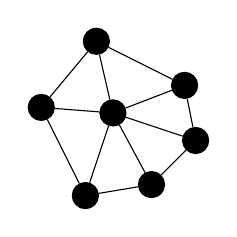
\begin{tikzpicture}[scale=.7,every node/.style={draw,shape=circle,fill=black,minimum size=1pt}]
% vertices
\path (0.5,1.5) node (p0) {}
(0,0) node (p1) {}
(1.2,0.2) node (p2) {}
(2,1) node (p3) {}
(1.8,2) node (p4) {}
(0.2,2.8) node (p5) {}
(-0.8,1.6) node (p6) {};
% edges
\draw (p0) -- (p1)
(p0) -- (p2)
(p0) -- (p3)
(p0) -- (p4)
(p0) -- (p5)
(p0) -- (p6)
(p1) -- (p2)
(p2) -- (p3)
(p3) -- (p4)
(p4) -- (p5)
(p5) -- (p6)
(p6) -- (p1);
\end{tikzpicture}
\quad
\onslide<2-5> 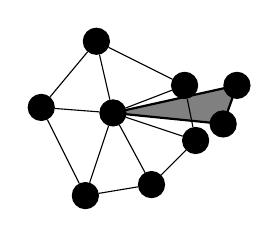
\begin{tikzpicture}[scale=.7,every node/.style={draw,shape=circle,fill=black,minimum size=1pt}]
\draw [fill=gray,thick] (0.5,1.5) -- (2.5,1.3) -- (2.75,2) -- (0.5,1.5);
% vertices
\path (0.5,1.5) node (p0) {}
(0,0) node (p1) {}
(1.2,0.2) node (p2) {}
(2,1) node (p3) {}
(1.8,2) node (p4) {}
(0.2,2.8) node (p5) {}
(-0.8,1.6) node (p6) {}
(2.5,1.3) node (p7) {}
(2.75,2) node (p8) {};
% edges
\draw (p0) -- (p1)
(p0) -- (p2)
(p0) -- (p3)
(p0) -- (p4)
(p0) -- (p5)
(p0) -- (p6)
(p1) -- (p2)
(p2) -- (p3)
(p3) -- (p4)
(p4) -- (p5)
(p5) -- (p6)
(p6) -- (p1);
\end{tikzpicture}
\quad
\onslide<3-5> 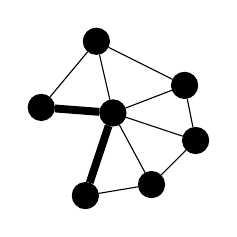
\begin{tikzpicture}[scale=.7,every node/.style={draw,shape=circle,fill=black,minimum size=1pt}]
% vertices
\path (0.5,1.5) node (p0) {}
(0,0) node (p1) {}
(1.2,0.2) node (p2) {}
(2,1) node (p3) {}
(1.8,2) node (p4) {}
(0.2,2.8) node (p5) {}
(-0.8,1.6) node (p6) {};
% edges
\draw (p0) -- (p1)
(p0) -- (p2)
(p0) -- (p3)
(p0) -- (p4)
(p0) -- (p5)
(p0) -- (p6)
(p1) -- (p2)
(p2) -- (p3)
(p3) -- (p4)
(p4) -- (p5)
(p5) -- (p6);
\draw [line width=.1cm] (p1) -- (p0) -- (p6);
\end{tikzpicture}
}
% bottom
\subfigure{
\onslide<4-5> 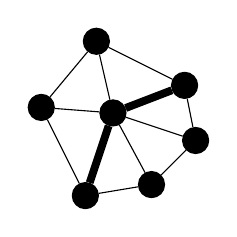
\begin{tikzpicture}[scale=.7,every node/.style={draw,shape=circle,fill=black,minimum size=1pt}]
% vertices
\path (0.5,1.5) node (p0) {}
(0,0) node (p1) {}
(1.2,0.2) node (p2) {}
(2,1) node (p3) {}
(1.8,2) node (p4) {}
(0.2,2.8) node (p5) {}
(-0.8,1.6) node (p6) {};
% edges
\draw (p0) -- (p1)
(p0) -- (p2)
(p0) -- (p3)
(p0) -- (p4)
(p0) -- (p5)
(p0) -- (p6)
(p1) -- (p2)
(p2) -- (p3)
(p3) -- (p4)
(p4) -- (p5)
(p5) -- (p6)
(p6) -- (p1);
\draw [line width=.1cm] (p1) -- (p0) -- (p4);
\end{tikzpicture}
\quad
\onslide<5> 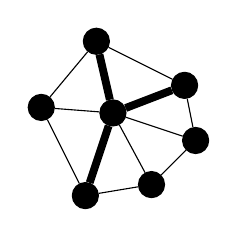
\begin{tikzpicture}[scale=.7,every node/.style={draw,shape=circle,fill=black,minimum size=1pt}]
% vertices
\path (0.5,1.5) node (p0) {}
(0,0) node (p1) {}
(1.2,0.2) node (p2) {}
(2,1) node (p3) {}
(1.8,2) node (p4) {}
(0.2,2.8) node (p5) {}
(-0.8,1.6) node (p6) {};
% edges
\draw (p0) -- (p1)
(p0) -- (p2)
(p0) -- (p3)
(p0) -- (p4)
(p0) -- (p5)
(p0) -- (p6)
(p1) -- (p2)
(p2) -- (p3)
(p3) -- (p4)
(p4) -- (p5)
(p5) -- (p6)
(p6) -- (p1);
\draw [line width=.1cm] (p1) -- (p0) -- (p4);
\draw [line width=.1cm] (p0) -- (p5);
\end{tikzpicture}
}	
\end{minipage}
\end{figure}
\end{frame}

\begin{frame}
\begin{itemize}
  \item \textbf{削减顶点引起的多边形减少~[Schroeder(1992)]}
  \begin{itemize}
    \onslide<1-2> \item 简单情形:削减前的多边形数量:$6$,削减后的多边形数量:$4$
    \onslide<2> \item 边缘情形:削减前的多边形数量:$5$,削减后的多边形数量:$4$
  \end{itemize}
\end{itemize}
\begin{figure}
\begin{minipage}[t]{0.8\linewidth}
\centering
% top
\subfigure{
\onslide<1-2> 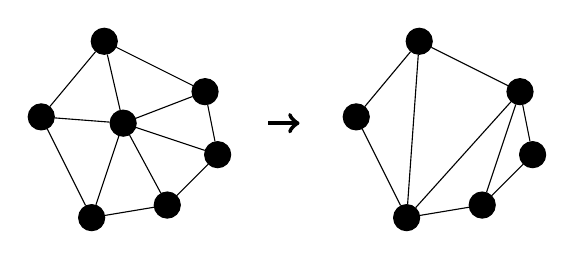
\begin{tikzpicture}[scale=.8,every node/.style={draw,shape=circle,fill=black,minimum size=3pt}]
% vertices
\path (0.5,1.5) node (p0) {}
(0,0) node (p1) {}
(1.2,0.2) node (p2) {}
(2,1) node (p3) {}
(1.8,2) node (p4) {}
(0.2,2.8) node (p5) {}
(-0.8,1.6) node (p6) {};
\path %(5.5,1.5) node (p7) {}
(5,0) node (p8) {}
(6.2,0.2) node (p9) {}
(7,1) node (p10) {}
(6.8,2) node (p11) {}
(5.2,2.8) node (p12) {}
(4.2,1.6) node (p13) {};
% edges
\draw (p0) -- (p1)
(p0) -- (p2)
(p0) -- (p3)
(p0) -- (p4)
(p0) -- (p5)
(p0) -- (p6)
(p1) -- (p2)
(p2) -- (p3)
(p3) -- (p4)
(p4) -- (p5)
(p5) -- (p6)
(p6) -- (p1);
\draw (p8) -- (p9)
(p9) -- (p10)
(p10) -- (p11)
(p11) -- (p12)
(p12) -- (p13)
(p13) -- (p8)
(p8) -- (p12)
(p8) -- (p11)
(p9) -- (p11);
% draw arrow
\draw [->,ultra thick] (2.8,1.5) -- (3.3,1.5);
\end{tikzpicture}
}
% bottom
\subfigure{
\onslide<2> 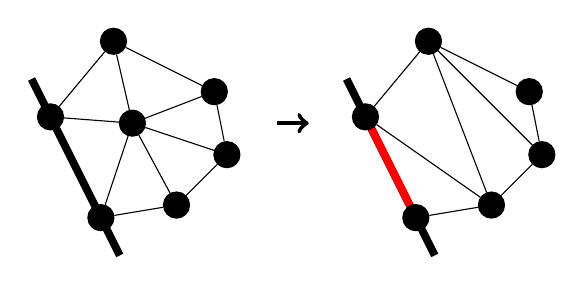
\begin{tikzpicture}[scale=.8,every node/.style={draw,shape=circle,fill=black,minimum size=3pt}]
% vertices
\path (0.5,1.5) node (p0) {}
(0,0) node (p1) {}
(1.2,0.2) node (p2) {}
(2,1) node (p3) {}
(1.8,2) node (p4) {}
(0.2,2.8) node (p5) {}
(-0.8,1.6) node (p6) {};
\path %(5.5,1.5) node (p7) {}
(5,0) node (p8) {}
(6.2,0.2) node (p9) {}
(7,1) node (p10) {}
(6.8,2) node (p11) {}
(5.2,2.8) node (p12) {}
(4.2,1.6) node (p13) {};
% edges
\draw (p0) -- (p1)
(p0) -- (p2)
(p0) -- (p3)
(p0) -- (p4)
(p0) -- (p5)
(p0) -- (p6)
(p1) -- (p2)
(p2) -- (p3)
(p3) -- (p4)
(p4) -- (p5)
(p5) -- (p6);
\draw [line width=0.1cm] (-1.1,2.2) -- (0.3,-0.6);
\draw (p8) -- (p9)
(p9) -- (p10)
(p10) -- (p11)
(p11) -- (p12)
(p12) -- (p13)
(p13) -- (p8)
(p9) -- (p13)
(p9) -- (p12)
(p10) -- (p12);
\draw [line width=0.1cm] (3.9,2.2) -- (5.3,-0.6);
\draw [line width=0.1cm,red] (p8) -- (p13);
% draw arrow
\draw [->,ultra thick] (2.8,1.5) -- (3.3,1.5);
\end{tikzpicture}
}	
\end{minipage}
\end{figure}
\end{frame}

\begin{frame}
\begin{itemize}
  \item \textbf{表面模型的VOI提取及连接性检验}:
\end{itemize}
\begin{figure}[t]
\centering
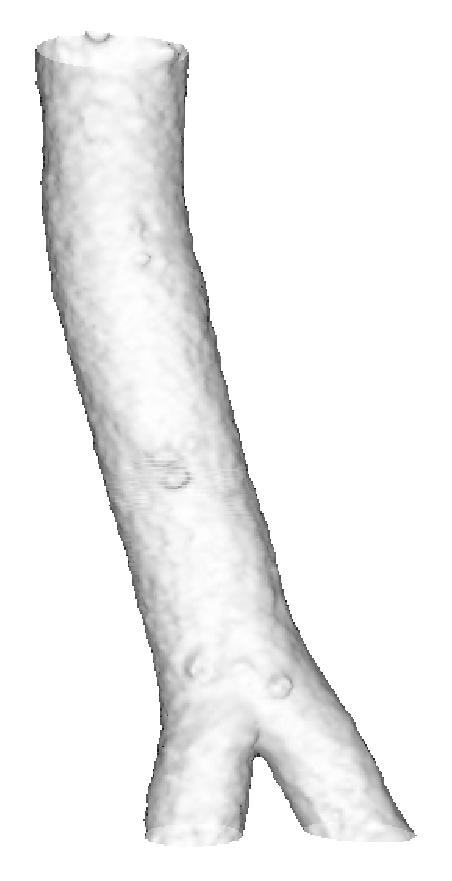
\includegraphics[height=2.0in]{../../Figures/postprocessing/mesh/original.eps}
\qquad
\raisebox{20mm}{
\centering
\renewcommand{\arraystretch}{0.5}
\begin{tabular*}{40mm}{lc}
\toprule
~                & \small{多边形数量} \\
\midrule
\small{检验前}   & \small{$74,307$}  \\
\small{检验后}   & \small{$74,307$}  \\
\bottomrule
\end{tabular*}
}
\end{figure}
% }
% \caption[表面模型的VOI提取及连接性检验]{表面模型的VOI提取及连接性检验。}
% \label{fig:mesh_connectivity}
\end{frame}

\begin{frame}
\begin{itemize}
  \item \textbf{设置不同参数获得的平滑结果}:($N$:迭代次数;$\delta$:带宽)
  \begin{itemize}
  \item \textbf{目的}:除去噪声,填补漏洞
  \end{itemize}
\end{itemize}
\begin{figure}[t]
\renewcommand{\arraystretch}{0.5}
% \caption[为平滑算法设置不同的参数所获得的结果]{为平滑算法设置不同的参数所获得的结果($N$:迭代次数;$\delta$:带宽)}
% \label{tbl:mesh_smooth}
\centering
\begin{tabular}{|l|c|c|c|}
\hline
\bigstrut ~                                   & \raisebox{-1mm}{$N = 30$}                                     & \raisebox{-1mm}{$N = 60$}                                     & \raisebox{-1mm}{$N = 100$}                                     \\
\hline
\bigstrut[t] \raisebox{0mm}{$\delta = 0.1$}  & \Includegraphics[height=1.0in]{../../Figures/postprocessing/mesh/smooth_30_1.eps}  & \Includegraphics[height=1.0in]{../../Figures/postprocessing/mesh/smooth_60_1.eps}  & \Includegraphics[height=1.0in]{../../Figures/postprocessing/mesh/smooth_100_1.eps}  \\
\hline
\bigstrut[b] \raisebox{0mm}{$\delta = 0.01$} & \Includegraphics[height=1.0in]{../../Figures/postprocessing/mesh/smooth_30_01.eps} & \Includegraphics[height=1.0in]{../../Figures/postprocessing/mesh/smooth_60_01.eps} & \Includegraphics[height=1.0in]{../../Figures/postprocessing/mesh/smooth_100_01.eps} \\
\hline
\end{tabular}
% \caption[设置不同参数获得的平滑结果(优化)]{设置不同参数获得的平滑结果。($N$:迭代次数;$\delta$:带宽)}
% \label{fig:mesh_smooth}
\end{figure}
\end{frame}

\begin{frame}
\begin{itemize}
  \item \textbf{设置不同参数获得的精简}:(精简率公式:$R = \frac{Q_r}{Q}$)
\end{itemize}
\begin{figure}[t]
\begin{table}[t]
\renewcommand{\arraystretch}{0.5}
% \caption[为削减算法设置不同参数所获得的结果]{为平滑算法设置不同的参数所获得的结果($N$:迭代次数;$\delta$:带宽)}
% \label{tbl:mesh_decimate}
\centering
\begin{tabular}{|l|c|c|c|}
\hline
\bigstrut ~                                    & \raisebox{-1mm}{$10\%$}                                                                 & \raisebox{-1mm}{$90\%$}                                                               & \raisebox{-1mm}{$99\%$}                                     \\
\hline
\bigstrut[t] \raisebox{0mm}{\small{表面模型}} & \Includegraphics[height=1.0in]{../../Figures/postprocessing/mesh/smooth_100_01_d10.eps}     & \Includegraphics[height=1.0in]{../../Figures/postprocessing/mesh/smooth_100_01_d90.eps}   & \Includegraphics[height=1.0in]{../../Figures/postprocessing/mesh/smooth_100_01_d99.eps}   \\
\hline
\bigstrut[b] \raisebox{0mm}{\small{线框模型}} & \Includegraphics[height=1.0in]{../../Figures/postprocessing/mesh/smooth_100_01_d10_w.eps}   & \Includegraphics[height=1.0in]{../../Figures/postprocessing/mesh/smooth_100_01_d90_w.eps} & \Includegraphics[height=1.0in]{../../Figures/postprocessing/mesh/smooth_100_01_d99_w.eps} \\
\hline
\end{tabular}
% \caption[设置不同参数获得的精简]{设置不同参数获得的精简:上排展示了削减率分别为$10\%$,$90\%$,$99\%$时的结果;下排展示了上排相应削减结果所对应的线框表示。}
% \label{fig:mesh_decimate}
\end{table}
\end{figure}
\end{frame}

\begin{frame}
\begin{itemize}
  \item \textbf{削减率与削减后的多边形数量}:
\end{itemize}
\begin{table}[h]
\renewcommand{\arraystretch}{0.5}
% \caption[削减率与削减后的多边形数量]{削减率与削减后的多边形数量}
% \label{tbl:mesh_decimate}
\centering
\begin{tabular*}{90mm}{c r r r r r}
\toprule
% \bfseries      & \bfseries Quantity of polygonal surfaces \\
\hspace{2mm} \small{削减率 ($\%$)}  &     \small{$10$} &     \small{$50$} &     \small{$75$} &    \small{$90$} &  \small{$99$} \\
\midrule
\hspace{2mm} \small{多边形数量}     & \small{$66,875$} & \small{$37,153$} & \small{$18,576$} & \small{$7,430$} & \small{$743$} \\
\bottomrule
\end{tabular*}
\end{table}
\end{frame}

\begin{frame}
\begin{itemize}
\item \textbf{交互仿真的指标} (fps $=$ frames per second)
\begin{itemize}
\item \textbf{初始fps}:当虚拟导管进入血管模型时的fps值
\item \textbf{平均fps}:模型中心线上五个给定位置处fps的平均值
\item \textbf{成功}: 将虚拟导管推送至血管模型内部某个预设位置
\end{itemize}
\end{itemize}
\end{frame}

\begin{frame}
\begin{itemize}
  \item \textbf{精简率与fps——情形I}:本章实验模型
\end{itemize}
\begin{table}[t]
\renewcommand{\arraystretch}{0.5}
% \caption[精简率与fps——情形I]{精简率与fps——情形I}
% \label{tbl:mesh_FPS1}
\centering
\begin{tabular*}{90mm}{c r r r r r}
\toprule
\hspace{5mm} \small{精简率($\%$)}           & \small{$10$} & \small{$50$} & \small{$75$} & \small{$90$} & \small{$99$} \\
\midrule
\hspace{5mm} \small{仿真初始fps}              & \small{$30$} & \small{$35$} & \small{$38$} & \small{$41$} & \small{$42$} \\
\midrule
\hspace{5mm} \small{仿真平均fps}              &  \small{$6$} & \small{$10$} & \small{$15$} & \small{$18$} & \small{$30$} \\
\midrule
\hspace{5mm} \small{是否完成仿真?(是/否)}  &  \small{否}  &  \small{否}  & \small{是}   & \small{是}   & \small{是}   \\
\bottomrule
\end{tabular*}
\end{table}
\end{frame}

\begin{frame}
\begin{itemize}
  \item \textbf{精简率与fps——情形II}:完整血管模型
\end{itemize}
\begin{table}[t]
\renewcommand{\arraystretch}{0.5}
% \caption[精简率与fps——情形II]{精简率与fps——情形II}
% \label{tbl:mesh_FPS2}
\centering
\begin{tabular*}{80mm}{c r r r r r}
\toprule
\hspace{5mm} \small{精简率($\%$)}           & \small{$90$} & \small{$95$} & \small{$99$} \\
\midrule
\hspace{5mm} \small{仿真初始fps}              & \small{$20$} & \small{$32$} & \small{$31$} \\
\midrule
\hspace{5mm} \small{仿真平均fps}              &  \small{$4$} &  \small{$6$} & \small{$11$} \\
\midrule
\hspace{5mm} \small{是否完成仿真?(是/否)}  &  \small{否}  &  \small{否}  & \small{是}   \\
\bottomrule
\end{tabular*}
\end{table}
\end{frame}

% \begin{frame}

% \end{frame} 